\chapter{TurtleBot Gazebo Simulation}
\label{chap:TurtleBotGazeboSimulation}

\section{Quickstart Simulation}
\label{sec:QuickstartSimulation}

With this section, you should be able to start one of our TurtleBot Gazebo simulation environments. 

\subsection{Setting up your .bashrc file}
\label{ssec:bashrc}

You should have the the lines from Figure~\ref{fig:template_bashrc} inserted and adapted in your \verb$.bashrc$ file. The \verb$.bashrc$ file is located in your home folder. 
\begin{landscape}
  \begin{figure}[htbp]
    \begin{verbatim}
# ROS specific 
source /opt/ros/kinetic/setup.bash

# TurtleBots
ttbws_path=<insert your path to the ttbws folder here>

source ${ttbws_path}/devel/setup.bash

# ALICA/ttb_base specific stuff
export DOMAIN_FOLDER=${ttbws_path}/src/cnc-turtlebots/
export DOMAIN_CONFIG_FOLDER=${DOMAIN_FOLDER}/etc

# for loading the right models (environment and robot)
export GAZEBO_MODEL_PATH=${GAZEBO_MODEL_PATH}:${ttbws_path}/src/turtlebot/turtlebot_bringup/models
export TURTLEBOT_STACKS=ninja-hexagons
export TURTLEBOT_3D_SENSOR=ninja-kinect

#fancy prompt that also shows the current git branch
export PS1='\[\033[01;32m\]\u@\h\[\033[01;34m\] \w \[\033[01;31m\]$(__git_ps1 "[%s]")\[\033[01;34m\]\$\[\033[00m\] '
    \end{verbatim}
    \caption{Template for your .bashrc}
    \label{fig:template_bashrc}
  \end{figure}
\end{landscape}

Don't forget to close the terminal after you edited the \verb$.bashrc$ file. It will only be reloaded after you reopen the terminal or you type \verb$. .bashrc$ into each of the currently open consoles.

\subsection{Starting Gazebo Simulation}
\label{ssec:StartSimulation}

Currently, there are three different start-up scripts \textemdash each for another more or less complex environment. 

\begin{description}
  \item[simulation.launch] This is the most simple scenario. Except from the robot(s), there is only one model in the world. This model represents the walls and ground of our Distributed Systems Department.
  \item[disaster.launch] This scenario is very similar to the simulation.launch scenario. It simple includes further models with simple geometry. The idea is to represent some fire, gas, victims and landmarks for relative orientation. The scenario was used for a proof-of-concept in the \href{http://www.uni-kassel.de/eecs/fachgebiete/vs/research/nicer.html}{NICER project} and Stefan Niemczyk's disseration. 
  \item[service\_robots.launch] This scenario is currently the most complex scenario. It includes doors, that can be opened and closed via ROS messages. The rooms are filled with furnitures like tables and cupboards and a lot of items are lying arround, e.g., coke cans, trash cans, cups, tools, books, etc. Therefore, the world includes several Gazebo plugins for the doors to move, or the simulated robot arm to grasp things.
\end{description}

In order launch one of the scenarios, you need to execute the following command on your commandline:

\verb$roslaunch turtlebot_bringup <name-of-scenario>.launch$

In order to make the robot move arround, you need to execute the next command in another terminal:

\verb$roslaunch turtlebot_bringup navigation_gazebo.launch$

It will start the fake\_localization and move\_base node, which are responsible for localizing the robot in simulation and moving the robot arround, respectively.

For debugging purposes ROS provides us with the Robot Vizualization program (rviz). We have an already configured launch file for rviz:

\verb$roslaunch turtlebot_bringup rviz_sim.launch$

With rviz you are able to make the robot move arround and see what the robot sees.

\section{Simulation Environment}
\label{sec:SimulationEnvironment}

The different simulation environments of Gazebo are denoted as worlds. The worlds we developed are located in the \emph{world} folder of the \emph{turtlebot\_bringup} ROS package. Currently there exist three worlds: \emph{distributed\_system\_simple.world}, \emph{distributed\_sys\-tems\_com\-plex.world}, \emph{distributed\_systems\_disaster.world}. The simple world only includes the walls of the floor of the Distributed Systems department. In the complex version of it, furniture and several items are added for a more realistic simulation environment. The disaster world is an evaluation environment for the \href{http://www.uni-kassel.de/eecs/fachgebiete/vs/research/nicer.html}{NICER project} and not of further interest for this lecture. 

The world files are formatted in a custom XML format, denoted as SPF. The format is relatively well documented on its \href{http://sdformat.org}{project homepage}. Please note the different available versions of the format. In the world file the world's properties are specified. These properties include physic properties, lighting, atmosphere, wind, etc. Furthermore different models can be inserted into the world. Therefore, other files can be referenced in the world file. The following lines, e.g., place a model instance of a small table at the given position. The instance can later we referenced by its given name.

\begin{Verbatim}[fontsize=\small]
<model name='r1411_small_table'>
  <pose frame=''>0.77 4.46 0 0 0 0</pose>
  <include>
    <uri>model://small_table</uri>
  </include>
</model>
\end{Verbatim}

The line \verb$<uri>model://small_table</uri>$ is a where the magic happens. The protocol of this URI (\verb$model://$) states that the model needs to be found in a collection of locations given by the \verb$GAZEBO_MODEL_PATH$ environment variable (see Section~\ref{ssec:bashrc}). Taking a look at the \emph{models} folder in the \emph{turtlebot\_bringup} ROS package, you will find one folder per model. Each folder includes a \emph{.config} file and maybe several version of \emph{.spf} files for the model. The \emph{.config} file includes meta data about the model and references the different existing \emph{.spf} version files. In the \emph{.spf} files the model itself is specified, according to the \href{http://sdformat.org/spec?ver=1.6&elem=model}{SPF Model Specification}.

There exist several neat features in the SPF format. Especially, it is possible to include Ruby code, in order to automatically generate parts of models or worlds. Nevertheless a robot itself is seldom specified directly in the SPF format. Instead it is spawned at run-time into the simulation environment by an extra spawning process denoted as \emph{spawn\_model} that is part of the \emph{gazebo\_ros} package. The arguments for the spawning process is a description of the robot model given in the Unified Robot Description format (URDF). Documentation for this format are given by the corresponding \href{http://wiki.ros.org/urdf/Tutorials}{URDF package pages}. URDF is actually deprecated an should be replaced by SDF, but for legacy reasons it still exists (see \href{http://answers.gazebosim.org/question/62/sdf-vs-urdf-what-should-one-use/}{ROS Answer Post}). If it should happen to you, that you are in the need of changing something at a robot model that is specified in URDF, the \href{http://gazebosim.org/tutorials/?tut=ros_urdf}{Gazebo Tutorial about URDF} could become handy, too.

\section{TurtleBot Topics}
\label{sec:TurtleBotTopics}

At this point it is expected that you have profound understanding of ROS topics and the corresponding commandline tools. The purpose of this section is to help investigating or debugging typical topic errors related with our TurtleBot simulation environment. Furthermore, the most interesting topics are listed and explained.

\subsection{Investigating Topics}
\label{ssec:Investigating Topics}

The first approach is always to see which topics are available in your running system. Therefore, type \verb$rostopic list$ into your terminal. The output looks like this:

\begin{Verbatim}[fontsize=\scriptsize]
  /clock
  /gazebo/link_states
  /gazebo/model_states
  /gazebo/parameter_descriptions
  /gazebo/parameter_updates
  /gazebo/set_link_state
  /gazebo/set_model_state
  /leonardo/amcl/parameter_descriptions
  /leonardo/amcl/parameter_updates
  /leonardo/amcl_pose
  /leonardo/camera/depth/camera_info
  /leonardo/camera/depth/image_raw
  /leonardo/camera/depth/points
  /leonardo/camera/parameter_descriptions
  /leonardo/camera/parameter_updates
  /leonardo/camera/rgb/camera_info
  /leonardo/camera/rgb/image_raw
  ...
\end{Verbatim}

Much more information can be gained with the verbosity option of the same command: \verb$rostopic list -v$. Now the output is distinguished in published topics and subscribed topics, including the corresponding numbers of publishers and subscribers currently registered at the rosmaster process. As you should already know, the rosmaster process is the central ROS communication registry. It is spawned by the roscore process which in turn is spawned by any roslaunch process in case roscore is not running already. Here is an example for the verbatim output:


\begin{Verbatim}[fontsize=\scriptsize]
  Published topics:
  * /map_metadata [nav_msgs/MapMetaData] 1 publisher
  * /leonardo/move_base/local_costmap/obstacle_layer/parameter_updates [dynamic_reconfigure/Config] 1 publisher
  * /leonardo/move_base/local_costmap/footprint [geometry_msgs/PolygonStamped] 1 publisher
  * /leonardo/odom [nav_msgs/Odometry] 1 publisher
  ...
  
  Subscribed topics:
  * /leonardo/cmd_vel_mux/input/teleop [geometry_msgs/Twist] 1 subscriber
  * /gazebo/set_link_state [gazebo_msgs/LinkState] 1 subscriber
  * /tf [tf2_msgs/TFMessage] 2 subscribers
  * /leonardo/move_base/global_costmap/footprint [geometry_msgs/PolygonStamped] 1 subscriber
  * /leonardo/scan_hokuyo [sensor_msgs/LaserScan] 2 subscribers
  ...
\end{Verbatim}

As you may have noticed, the message type of each topic is given in square braces. Gaining this information that way, is sometimes much faster than surfing to the corresponding ROS documentation website.

One typical error, during programming your own ROS node, is that the topics of your node are not prefixed with the name of your robot at hand. When your node is working and is integrated into one of our launch files above the topics will be prefixed automatically, but if you test your node ``by hand'' you have to take care by yourself, that the topics include the robots name (if necessary). The prefixes are necessary, for example, in order to have one path planning topic for each spawned robot. Otherwise all robots would receive the same path planning goals and drive to them. 

Another option is to run rqt\_graph from the commandline. It will open a sophisticated GUI, that visualize the current ROS topic graph and is able to update at runtime. We recommand to visualize nodes and topics \textendash in this case nodes are ellipses and topics are rectangles. Hovering above some node, will highlight sending and receiving topics of that node.

\section{Moving arround with Move Base}
\label{sec:MovingWithMoveBase}

In this section, we document our experience with the motion framework in ROS, including \href{http://wiki.ros.org/move_base}{move base}, \href{http://wiki.ros.org/dwa_local_planner}{local} and \href{http://wiki.ros.org/global_planner}{global} pathplanner, \href{http://wiki.ros.org/costmap_2d}{local and global costmap}, \href{http://wiki.ros.org/fake_localization}{fake localization}, and different submodules of the framework.

\subsection{Fake Localization}
\label{ssec:FakeLocalization}

Moving arround requires to be localized. In a simulated environment, we are in the lucky situation that the simulator provides us with a perfect position allowing to omit any extra localization algorithm, e.g., the Adaptive Monte Carlo Localization (AMCL). Two things are necessary, for a perfect localization through the simulator itself. First we need to load a certain plugin into the gazebo runtime. Therefore, we inserted the following lines into the file \verb$turtlebot_description/urdf/turtlebot_gazebo.urdf.xacro$:

\begin{Verbatim}[fontsize=\scriptsize]
 <!-- Makes Gazebo publishing a ground truth position. -->
  <xacro:macro name="turtlebot_ground_truth_pose">
    <gazebo>
      <plugin name="p3d_controller" filename="libgazebo_ros_p3d.so">
       <alwaysOn>true</alwaysOn>
       <updateRate>100.0</updateRate>
       <bodyName>base_link</bodyName>
       <topicName>ground_truth_pose</topicName>
       <frameName>/map</frameName>
       <xyzOffsets>1 1 0</xyzOffsets> <!-- option to initialize odometry for fake localization-->
       <rpyOffsets>0 0 0</rpyOffsets>
      </plugin>
    </gazebo>
  </xacro:macro>
\end{Verbatim}

In future, this xacro needs additional parameters,e.g., setting the xyzOffsets according to the intial robots position. In order to use this xacro we inserted the following line into the \verb$turtlebot_description/robots/kobuki_ninja-hexagons_ninja-kinect_sim.urdf.xacro$ file:

\verb$<turtlebot_ground_truth_pose/>$

At this point the simulator is already pubishing the ground-truth position of each roboto to the topic \emph{$<$robotname$>$/ground\_truth\_pose}, but this is not very compatible to the downstream packages running on real and simulated robots. Therefore we introduced the actual \verb$fake_localization$ node into the \verb$navigation_gazebo.launch$ start-up script, like this:

\begin{Verbatim}[fontsize=\scriptsize]
<!-- Localization -->
<node pkg="fake_localization" type="fake_localization" name="fake_localization">
 <param name="odom_frame_id"   value="/leonardo/odom"/>
 <param name="base_frame_id"   value="/leonardo/base_link"/>
 <remap from="base_pose_ground_truth" to="ground_truth_pose"/>
</node>
\end{Verbatim}

This \verb$fake_localization$ node will us the simulators ground-truth position and publish this position like AMCL would do. This makes the localization compatible to move base and any other common motion package in ROS. 

\subsection{Move Base}
\label{ssec:MoveBase}

Move Base is a single ROS node, as you would expect it to be for a single purpose (move arround) component. Nevertheless, it comprises a rather complex set of components, like different costmaps, and path planners. There exists a rather \href{http://wiki.ros.org/move_base}{verbose documentation} about the architecture of Move Base, we recommend to read it! Further informations can be gathered from a nice \href{http://kaiyuzheng.me/documents/navguide.pdf}{report about tuning Move Base} and its components from Kaiyu Zheng (2016). You should definitely read it, too.

\paragraph{Path Planners}

For the local and global path planner, we followed the tuning guide and did choose the \href{http://wiki.ros.org/global_planner}{global\_planner} as global path planner and the \href{http://wiki.ros.org/dwa_local_planner}{dwa\_local\_planner} as local path planner. 

\paragraph{Cost Maps}

The software for the local and global costmap is basically the same: \href{http://wiki.ros.org/costmap_2d}{costmap\_2d}. The crucial difference is located it is configuration files. Apart from looking at the configuration files (located in \verb$turtlebot_bringup/param/$), we recommend again to read the \href{http://kaiyuzheng.me/documents/navguide.pdf}{tuning guide} from Kaiyu Zheng.

\paragraph{Simple Move Base Interface}

Interacting with the move\_base node is a little bit complex, as it uses an \href{http://wiki.ros.org/actionlib/Tutorials}{ROS Action Server}. For simply posting a path planning goal to move\_base you can use the topic \verb$/leonardo/move_base_simple/goal$. The move\_base node will drive to that goal without giving you feedback about it. 

\subsection{Additional Components}
\label{ssec:AddComponents}

Additional to Move Base, there exist several auxiliary ROS nodes, concerned about the motion of a robot:

\begin{description}
  \item[Safety Controller:] A safetry controller, is some low-level piece of software that should avoid any dangerous action of the robot, like falling down some stairs or driving against sensitive objects or humans. Therefore, it is subscribed to certain sensor topics and publishes risk avoiding movement commands, i.d., stop when there is a cliff in your current direction, drive backwards when you hit something, etc. Currently there exist at least two safety controlle, that a rather similar: \href{http://wiki.ros.org/kobuki_safety_controller}{kobuki\_safety\_controller}, \href{http://wiki.ros.org/yocs_safety_controller}{yocs\_safety\_controller}.
  \item[Velocity Muxer:] This simple node is an arbiter that decides which of its subscribed motion command topics should be forwarded to the actual robot hardware or simulator. It does this simply be a given priority for each subscribed topic. The safety controlle, e.g., should have the highest priority, while normal moving commands can have a lower priority. This guarantees, e.g., that the robot's hardware or simulator does not receive movement commands in different directions at the same time. Here is the \href{http://wiki.ros.org/cmd_vel_mux}{documentation of the muxer}.
  \item[Velocity Smoother:] The \href{http://wiki.ros.org/yocs_velocity_smoother}{velocity smoother} tries to avoid jumps in movement commands and the robot's actual movements. Therefore, it applies configured limits to the incoming motion commands and prohibits accelerations and velocities beyond the hardware limits of a robot. 
\end{description}

In our simulation environment, we decided to drop all of these additional components and let the Move Base node talk to the simulator directly.

\section{Turtlebot Sensor Plugin}

To simulate various scenarios using the TurtleBot there was a need for a more specific and configurable type of sensor. We developed a sensor plugin for gazebo to accomplish that. It allows the user to configure detection angles, range and the type of object in a configuration file. You may think of it, as a laser scanner sensor, that can reach through walls and perfectly detects what ever it was specified for.

\subsection{Configuration}

The configuration format uses a similar syntax as the configuration for the ProcessManager mentioned in Section~\ref{chap:ProcMan}.

The file itself is located at the configuration path defined by the \verb$DOMAIN_CONFIG_FOLDER$ environement variable (see Section~\ref{ssec:bashrc}) and has the filename \textit{LogicalCamera.conf}.

Let's take a look at the following example configuration:

\begin{verbatim}
[LogicalCamera]
        [Victim]
                # meter
                range = 3
                type = victim
                # Hz
                publishingRateHz = 1

                # angles have to be set from 180 to -180 degree
                [DetectAngles]
                        [Front]
                                startAngle = -135
                                endAngle = 135
                        [!Front]
                [!DetectAngles]
        [!Victim]
        [Fire]
                # meter
                range = 5
                type = fire
                # Hz
                publishingRateHz = 10

                # angles have to be set from 180 to -180 degree
                [DetectAngles]
                        [Front]
                                startAngle = -180
                                endAngle = 180
                        [!Front]
                [!DetectAngles]
        [!Fire]
[!LogicalCamera]
\end{verbatim}

The first Block \verb$[LogicalCamera]$ is the uppermost block and has to be followed by \verb$[!LogicalCamera]$ at the end.

In this example we want to detect two types of objects. The first one is the presence of victims and the second one is fire. Each distinct type has to be defined as a block, similar to the uppermost LogicalCamera Block. Hence we have \verb$[Victim] ... [!Victim]$ and \verb$[Fire] ... [!Fire]$ here.

In these type blocks, we now have to define the properties of the sensor for that given type of object.

Here, a victim can be detected in a \textbf{range} of 3 meters, as given to  the range parameter.

The \textbf{type} parameter is used by the plugin to determine which object belongs to which type. The plugin filters these types depending on the objects name in gazebo. So an object called \textit{victim\_box} is going to be detected as a victim type object.

Using the parameter \textbf{publishingRateHz} as the name suggests you can set the rate in which an object may be detected. A victim will be only detected once a second, while a fire can be detected up to ten times a second.

Next, the block \textbf{DetectAngles} allows you to specify multiple sections in which the robot can detect the object.

Angles have to be in a range from -180° to 180°.

Figure~\ref{fig:TurtleBotSensorAngles} shows how the angles have to be speciefied.

\begin{figure}[htbp]
  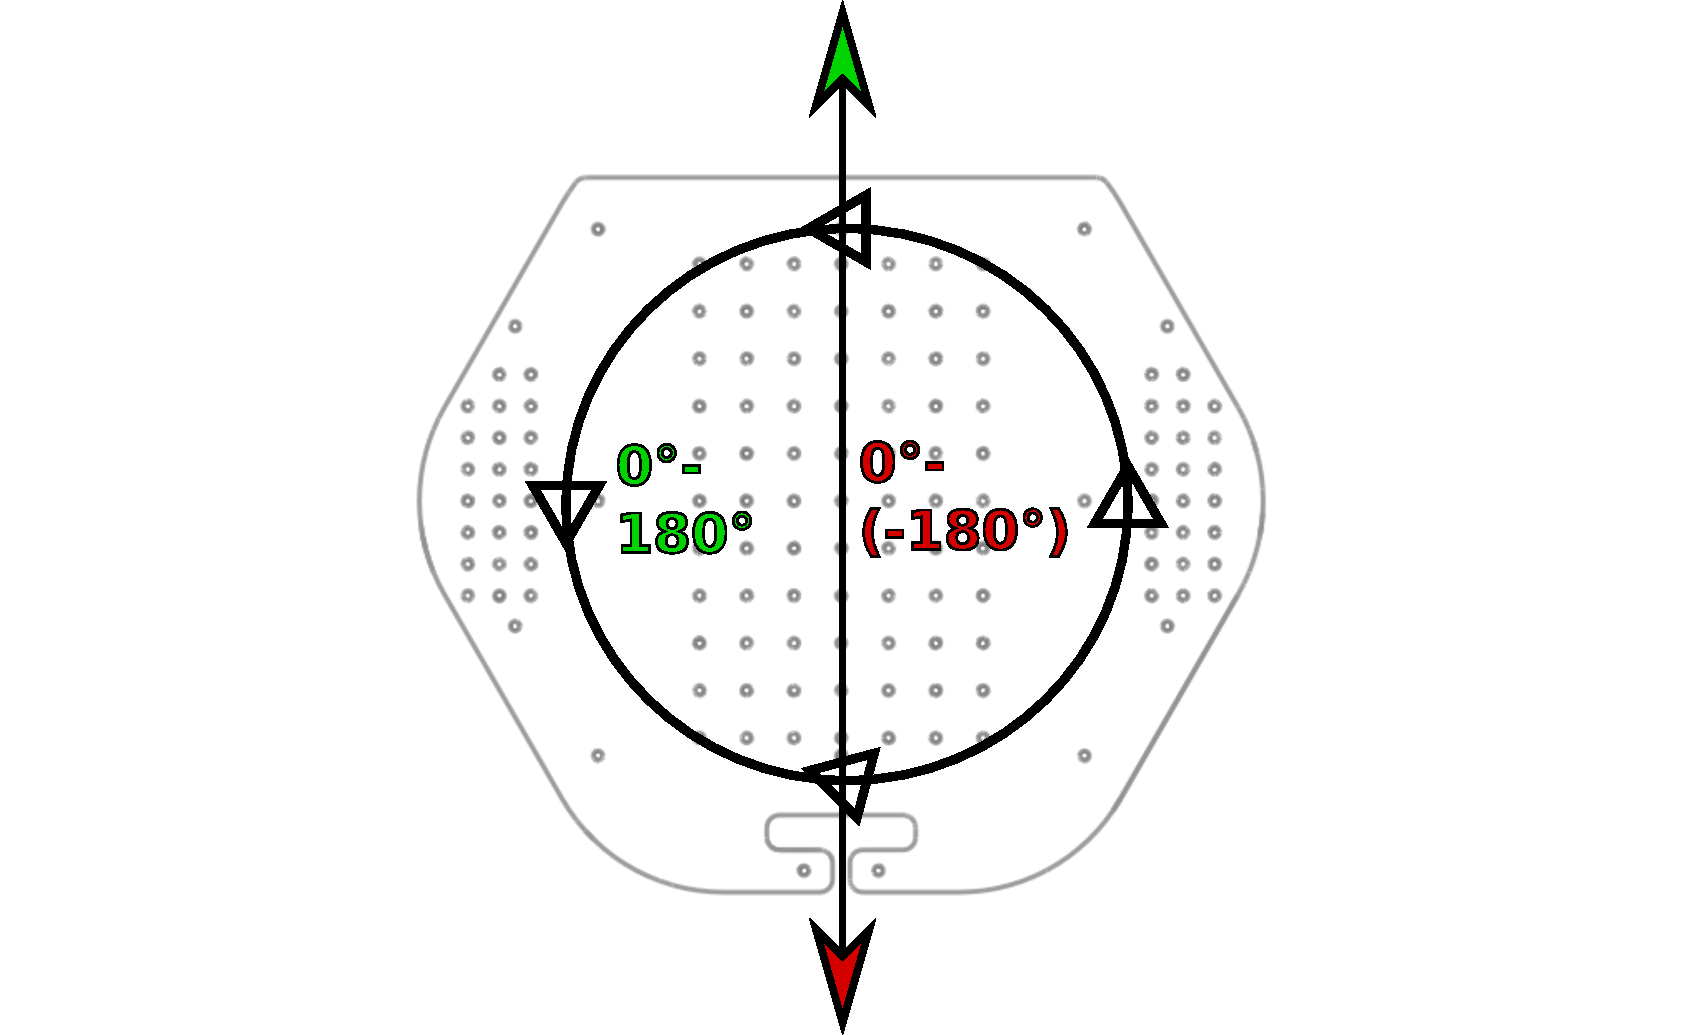
\includegraphics[width=1.0\textwidth]{ttbangles.pdf}
  \caption{How to specify the sensor angles}
  \label{fig:TurtleBotSensorAngles}
\end{figure}

\subsection{Sensor message}

Every time an object has been detected according to the configuration, a ROS message gets sent.

The name of the ros topic is \verb$logical\_camera$ and is namespaced with the robot name, as configured in the \textit{robot.simulation} file. So for a robot named leonardo, the message will get published on the topic  /leonardo/logical\_camera.

The message itself has the following fields:

\verb$string modelName$

Name of the detected model/object in gazebo

\verb$geometry\_msgs/Pose2D pose$

Posoition of the object on the x,y plane(map seen from top)

\verb${ObjectSize size$

Approximate size of an object. Contains fields xsize, ysize and zsize.

\verb$time timeStamp$

Time, when the object was detected.

\verb$string type$

Object type. See Configuration Section for details.

\subsection{Robot coordinate system}

Looking from the top at the turtlebot, the coordinate system looks like shown in Figure~\ref{fig:TurtleBotCoordinates}.
\begin{figure}[htbp]
  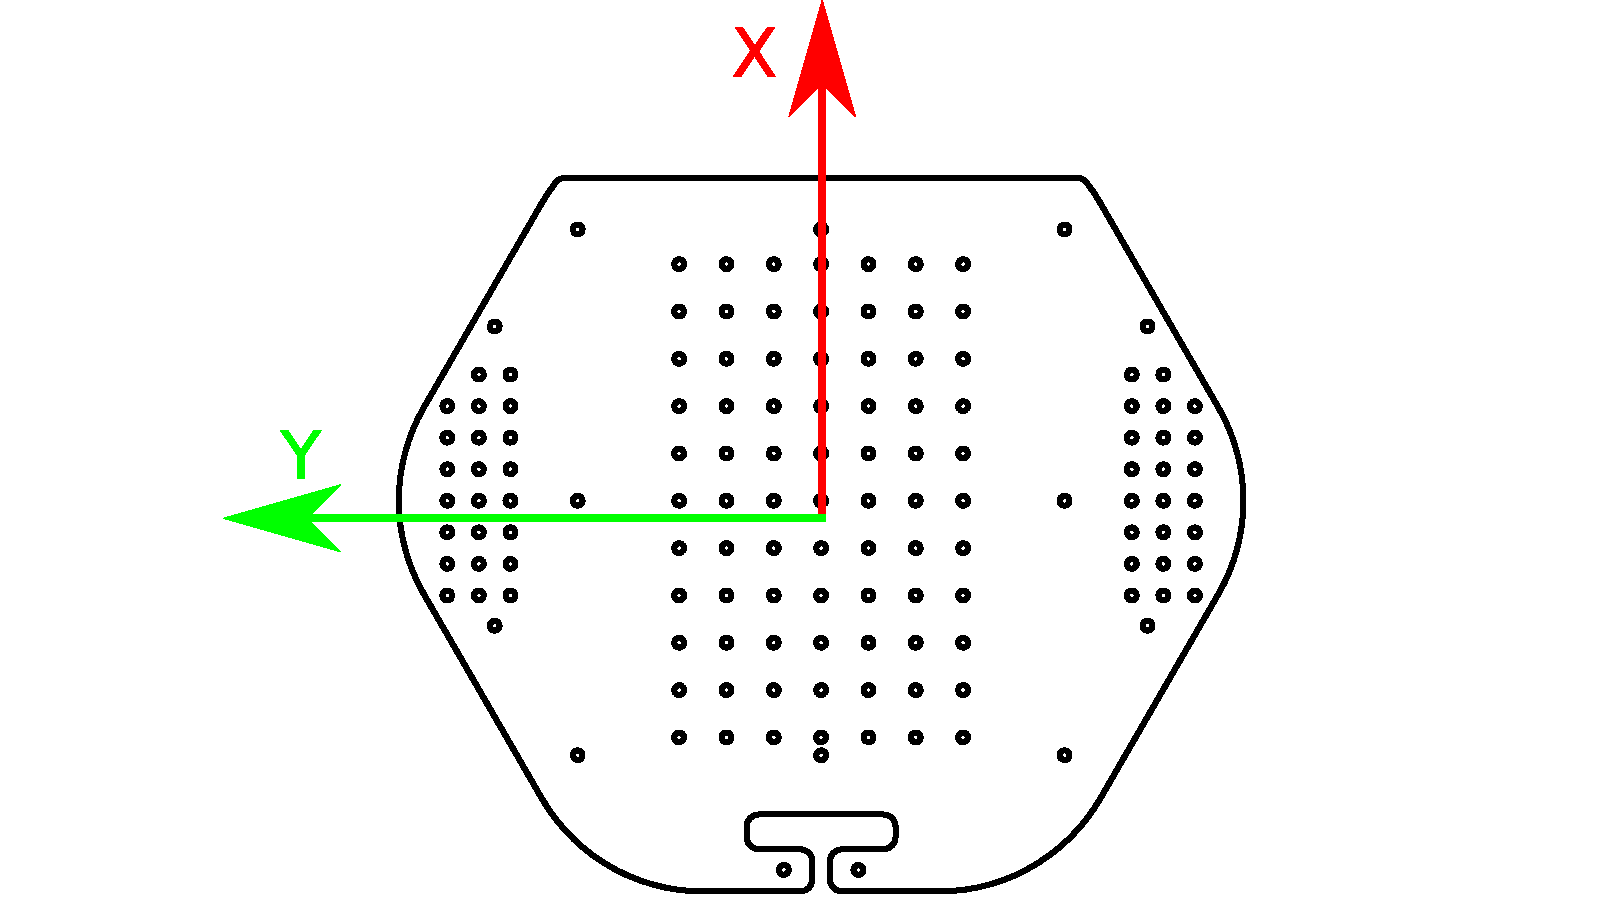
\includegraphics[width=1.0\textwidth]{ttbtop.pdf} 
  \caption{The TurtleBot Coordinate System}
  \label{fig:TurtleBotCoordinates}
\end{figure}

So the a positive X coordinate means, an object is ahead of the robot, while a negative one means, it is behind the robot. In the same way, a positive Y means that an object is detected left of the robot, while a positive Y coordinate means that it was detected on the right side.

As a side note, the Z coordinate tells you how high is an object in relation to the sensor. A positive Z means, that the object is above the sensor, while a negative Z means, that it is negative.

\subsection{Using the sensor plugin in gazebo}

First, make sure you configured the plugin as described in the configuration section.

Then simply launch gazebo using the simulation launch file:

\begin{verbatim}
roslaunch turtlebot_bringup simulation.launch
\end{verbatim}

In order for the plugin to correctly detect and filter the objects, you have to give each object a name, that contains the type string from the configuration. A \textit{victim\_box} may for example be detected  as a victim or box type of object.

Now, to add objects in Gazebo you can for example add a cube using the cube button in toolbar on top of the 3D view. For more information about adding objects in gazebo, take a look at the corresponding gazebo tutorial.

To quickly test the sensor you can add a cube or sphere and rename it as follows.  First, add an object using the cube, sphere or cylindar button in the top bar. Then select the object by left clicking on it and then right click it to bring up the context menu. In the menu select \textit{Edit Model}. You are now in the Model Editor. In the left Pane select the Model Tab and change the Model Name to a name that contains the type string. After you are done, exit the Model Editor by select \textit{Exit Model Editor} in the \textit{File Menu}.

Now you may have to continue the simulation by pressing the play button on the bar below the 3D view. After that you should be able to receive messages from the plugin on the \textit{logical\_camera} topic.